\def\fileversion{3.0}
\def\filename{jss}
\def\filedate{2015/09/01}
%
% \iffalse
%
%%
%% Package `jss' to use with LaTeX2e for JSS publications (http://www.jstatsoft.org/)
%% License: GPL-2 | GPL-3
%% Copyright: (C) Achim Zeileis
%% Please report errors to Achim.Zeileis@R-project.org
%%
%
% \fi
%
% \changes{0.1}{2004/08/09}
%   {First draft.}
%
% \changes{1.0}{2004/09/29}
%   {First release.
%    - new font size (11pt)
%    - better formatting of sections}
%
% \changes{1.1}{2004/10/01}
%   {Bug fix: sections and pdfbookmarks
%    (arguments were switched).}
%
% \changes{1.2}{2004/10/02}
%   {changed logo name, improved docs}
%
% \changes{1.3}{2004/10/05}
%   {fixed Shorttitle default}
%
% \changes{1.4}{2005/01/28}
%   {updated docs}
%
% \changes{1.5}{2005/12/09}
%   {now an official ASA journal}
%
% \changes{1.6}{2007/01/28}
%   {small enhancements}
%
% \changes{1.7}{2007/10/15}
%   {changed link colors, modifed hyperref inclusion for texlive}
%
% \changes{1.8}{2008/04/08}
%   {added option to omit JSS markup, slightly changed pkg markup}
%
% \changes{2.0}{2009/09/24}
%   {added GPL-2 license, new options 'notitle' and 'noheadings'}
%
% \changes{2.1}{2012/06/07}
%   {allow _ in doi, new option 'nofooter'}
%
% \changes{2.2}{2013/04/06}
%   {omit dependency on a4wide, hard-code page layout instead}
%
% \changes{2.3}{2013/09/05}
%   {added optional GPL-3 license}
%
% \changes{3.0}{2015/09/01}
%   {include DOI, list FOAS as publisher}
%
%
%
% \MakeShortVerb{\|}
% \newcommand{\foopkg}[1]{{\normalfont\fontseries{b}\selectfont #1}}
% \newcommand{\enquote}[1]{``#1''}
%
% \title{\foopkg{jss}: A Document Class for Publications in the Journal of Statistical Software}
% \author{Achim Zeileis}
%
% \maketitle
%
% \section{Introduction} \label{sec:intro}
%
% The \LaTeXe{} document class \foopkg{jss} is an extension of the
% standard \LaTeXe{} \foopkg{article} class for publications in the
% Journal of Statistical Software (JSS, \url{http://www.jstatsoft.org/}).
% Additionally, the JSS-specific header/footer can be easily switched
% off so that the document class can easily be used for other publications,
% e.g., \textsf{R} package vignettes.
%
% The document class provides infrastructure for all four kinds of publications
% in JSS: regular articles, code snippets, book reviews and
% software reviews. Each document requires several declarations to
% be made in the header (before |\begin{document}|) 
% which are described in Section~\ref{sec:ifa} separately
% for articles/code snippets and book/software reviews
% along with some general commands
% which can be used in all documents.
%
% The final version of JSS papers should be prepared using this JSS style file;
% the submission of the final version needs to include the full sources
% (|.tex|, |.bib|, and all graphics). A quick check for the most important aspects
% of the JSS style is given in Section~\ref{sec:check}; authors should make sure that all
% of them are addressed in the final version. A list of frequently asked questions
% (FAQ) is available online \url{http://www.jstatsoft.org/style} that provides
% additional details and tries to address typical problems.
%
% All documents need to be processed by pdf\LaTeX{}, some useful information
% on this is provided in Section~\ref{sec:TeX}, which also contains some
% information on using \textsc{Bib}\TeX{}. \textsc{Bib}\TeX{} together
% with the style file |jss.bst| produces references
% and citations in the required format.
%
% The actual code for the batch file (|jss.ins|), the
% driver (|jss.drv|) and the class (|jss.cls|) are
% briefly described in Section~\ref{sec:code}. Note, that usually
% you do not have to read that section when you want to prepare
% a submission for JSS.
%
%
% \section{Instructions for authors} \label{sec:ifa}
%
% To use the JSS styles, you have to include the class file
% |jss.cls|, the logo |jsslogo.jpg| and the \textsc{Bib}\TeX{}
% style \texttt{jss.bst} in your search path. This can either be
% your local working directory or in your |texmf| or 
% |localtexmf| tree.
%
% The \LaTeX{} documents have to include the |jss.cls| first by
% 
% |\documentclass[|\textit{type}|]{jss}|
% 
% where \textit{type} can be |article| (which is the default),
% |codesnippet|, |bookreview| or |softwarereview|.
% Templates with brief instructions are provided in
% |article.tex|, |codesnippet.tex|, |bookreview.tex|
% and |softwarereview.tex| respectively. The corresponding
% commands used for the header declarations are described
% in more detail in the following.
%
% By using |jss.cls|, the packages \foopkg{graphicx},
% \foopkg{color}, \foopkg{hyperref}, \foopkg{ae}, \foopkg{fancyverb} and
% \foopkg{natbib} are loaded automatically.
% Authors may, of course, include further packages
% but should not change the page layout
% or change the font or font encoding. If the package \foopkg{thumbpdf}
% is available, its inclusion is encouraged.
%
% The titles of JSS publications are capitalized, i.e., in title style, but the section
% headers are not and should be in sentence-style.
%
% Acknowledgments should be included at the end of the paper before the
% references in a separate section set up via |\section*{Acknowledgments}|.
%
% \emph{Hint.} If you want to use markup in section headers you will usually
% have to escape it for the PDF bookmarks by giving the text for the 
% bookmark explicitly without markup, e.g.,
% \begin{verbatim}
% \section[Calling C++ from R]{Calling \proglang{C++} from \proglang{R}}
% \end{verbatim}
%
% \emph{Hint.} If compilation with pdf\LaTeX{} fails with an error at
% |\begin{document}| the reason is almost surely that some of the
% declarations in the header have not been made properly. For example,
% |\Plainauthor|, |\Plaintitle| or |\Plainkeywords| might be missing
% or still containing markup.
%
% \emph{Hint.} If you want to use the JSS style for a non-JSS paper
% (or a modification of a JSS paper, e.g., in a vignette), you can
% set the option |nojss| in the |\documentclass| statement to suppress
% JSS-specific layout.
%
% 
% \subsection{Style checklist} \label{sec:check}
% A quick check for the most important aspects of the JSS style is given below. 
% Authors should make sure that all of them are addressed in the final version.
% More details can be found in the remainder of this manual.
% 
% \begin{itemize}
%   \item The manuscript can be compiled by pdf\LaTeX{}.
%   \item |\proglang|, |\pkg| and |\code| have been used for highlighting
%         throughout the paper (including titles and references),
%         except where explicitly escaped.
%   \item References are provided in a |.bib| \textsc{Bib}\TeX{} database
%         and included in the text by |\cite|, |\citep|, |\citet|, etc.
%   \item Titles and headers are formatted properly:
%         \begin{itemize}
%           \item |\title| in title style,
%           \item |\section| etc.\ in sentence style,
%           \item all titles in the \textsc{Bib}\TeX{} file in title style.
%         \end{itemize}
%   \item Figures, tables and equations are marked with a |\label|
%         and referred to by |\ref|, e.g., ``|Figure~\ref{...}|''.
%   \item Software packages are |\cite{}|d properly.
% \end{itemize}
% 
% 
% \subsection{Articles and code snippets}
%
% For JSS articles and code snippets respectively, 
% the following declarations have to be made
% in the header of the \LaTeX{} sources (before |\begin{document}|).
% See also the template |article.tex| or |codesnippet.tex|
% respectively.
%
% \DescribeMacro{\author}
% The command |\author| specifies the list of authors. The name
% of each author should be followed by a linebreak and his
% affiliation (only the university, in a single line). The authors
% should be separated by |\And| (instead of |\and|), e.g.,
% \begin{verbatim}
% \author{Achim Zeileis\\Universit\"at Innsbruck \And 
%         Second Author\\Plus Affiliation}
% \end{verbatim}
% If not all authors fit into a single line, |\AND| (instead of
% |\And|) should be used in front of authors that should go into
% the next line.
% 
% \DescribeMacro{\Plainauthor}
% The list of authors without affiliations. It needs to be
% comma-separated and must not contain any markup (bold fonts etc.), e.g.,
% \begin{verbatim}
% \Plainauthor{Achim Zeileis, Second Author}
% \end{verbatim}
% 
% \DescribeMacro{\title}
% The title of the paper. It should be capitalized and may contain
% further markup (in particular markup such as |\pkg| and |\proglang|), e.g.,
% \begin{verbatim}
% \title{A Capitalized Title for a Package \pkg{foo}}
% \end{verbatim}
% 
% \DescribeMacro{\Plaintitle}
% The full title without any markup.
% The default is to use |\title|, therefore it needs to be specified
% only if it is different from |\title|, e.g.,
% \begin{verbatim}
% \Plaintitle{A Capitalized Title for a Package foo}
% \end{verbatim}
% 
% \DescribeMacro{\Shorttitle}
% A shorter version of the title to be used for page headings.
% The default is to use |\title|, therefore it needs to be specified
% only if it is different from |\title|, e.g.,
% \begin{verbatim}
% \Shorttitle{foo: A Capitalized Title}
% \end{verbatim}
% 
% \DescribeMacro{\Abstract}
% Enter the abstract for your article here, e.g.,
% \begin{verbatim}
% \Abstract{
%   The abstract of the article.
% }
% \end{verbatim}
% 
% \DescribeMacro{\Keywords}
% A comma-separated list of (at least one) keyword(s) which
% should not be capitalized, e.g.,
% |\Keywords{keywords, comma-separated, not capitalized}|.
%
% \DescribeMacro{\Plainkeywords}
% The list of keywords without any markup. The default is to use
% |\Keywords|, therefore it needs to be specified only
% if it is different from |\Keywords|.
%
% \DescribeMacro{\Volume}
% The JSS volume number in which the article is published,
% e.g., |\Volume{11}|. Note:
% This information will be provided upon acceptance
% or added by the technical editor. Prior to acceptance,
% do not use this command.
%
% \DescribeMacro{\Issue}
% The JSS issue number in which the article is published,
% e.g., |\Issue{9}|. Note:
% This information will be provided upon acceptance
% or added by the technical editor. Prior to acceptance,
% do not use this command.
%
% \DescribeMacro{\Month}
% The month in which the article is published,
% e.g., |\Month{September}|. Note:
% This information will be provided upon acceptance
% or added by the technical editor. Prior to acceptance,
% do not use this command.
%
% \DescribeMacro{\Year}
% The year in which the article is published,
% e.g., |\Year{2004}|. Note:
% This information will be provided upon acceptance
% or added by the technical editor. Prior to acceptance,
% do not use this command.
%
% \DescribeMacro{\Submitdate}
% The date of submission for the article,
% e.g., |\Submitdate{2004-09-29}|. Note:
% This information will be provided upon acceptance
% or added by the technical editor. Prior to acceptance,
% do not use this command.
%
% \DescribeMacro{\Acceptdate}
% The date of acceptance for the article,
% e.g., |\Acceptdate{2004-09-29}|. Note:
% This information will be provided upon acceptance
% or added by the technical editor. Prior to acceptance,
% do not use this command.
%
% \DescribeMacro{\Address}
% The address of (at least) one author should be given in
% the following format
% \begin{verbatim}
% \Address{
%   Achim Zeileis\\
%   Department of Statistics and Mathematics\\
%   Faculty of Economics and Statistics\\
%   Universit\"at Innsbruck\\
%   6020 Innsbruck, Austria\\
%   E-mail: \email{Achim.Zeileis@uibk.ac.at}\\
%   URL: \url{http://eeecon.uibk.ac.at/~zeileis/}
% }
% \end{verbatim}
% It is also possible to include your telephone and fax 
% number, by adding them in the format
% \begin{verbatim}
%   Telephone: +43/512/507-7103
%   Fax: +43/512/507-2851
% \end{verbatim}
% before the e-mail address.
%
% Furthermore, if the document is prepared using the |Sweave|
% functions in \textsf{R}, something like the following line
% \begin{verbatim}
% %% need no \usepackage{Sweave.sty}
% \end{verbatim}
% (with `\%\%') needs to be included in the header.
%
% \subsection{Book and software reviews}
%
% For JSS book and software respectively, 
% the following declarations have to be made
% in the header of the \LaTeX{} sources (before |\begin{document}|).
% See also the template |bookreview.tex| or |softwarereview.tex|
% respectively. Note that some commands might differ between
% book and software reviews, this is always stated explicitely
% below.
%
% \DescribeMacro{\Reviewer}
% The command |\Reviewer| specifies the name of the reviewer
% followed by a linebreak and his affiliation (only the university,
% in a single line), e.g.,
% \begin{verbatim}
% \Reviewer{Frederic Udina\\Pompeu Fabra University}
% \end{verbatim}
% 
% \DescribeMacro{\Plainreviewer}
% The name of the reviewer without affiliation. 
% It must not contain any markup (bold fonts etc.), e.g.,
% \begin{verbatim}
% \Plainauthor{Frederic Udina}
% \end{verbatim}
% 
% \emph{The following five commands are just required for book reviews.}
%
% \DescribeMacro{\Booktitle}
% The title of the book. It should be capitalized and may contain
% further markup (in particular markup such as |\pkg| and |\proglang|), e.g.,
% \begin{verbatim}
% \Booktitle{Visualizing Categorical Data}
% \end{verbatim}
%
% \DescribeMacro{\Bookauthor}
% Author(s) of the book, e.g.,
% \begin{verbatim}
% \Bookauthor{Michael Friendly}
% \end{verbatim}
% If there are several authors they should be comma-separated,
% and the last author separated by |and|, e.g.,
% |\Bookauthor{A and B}| or |\Bookauthor{A, B and C}|.
% 
% \DescribeMacro{\Pubyear}
% Year of publication, e.g., |\Pubyear{2000}|.
%
% \DescribeMacro{\ISBN}
% ISBN number, e.g., |\ISBN{1-58025-660-0}|.
%
% \DescribeMacro{\Pages}
% Number of pages, both arabic and roman (if available), e.g.,
% |\Pages{456}| or |\Pages{xvi + 145}|.
% 
% \emph{The following command is just required for software reviews.}
%
% \DescribeMacro{\Softwaretitle}
% The title of the software. It should be capitalized and may contain
% further markup (in particular markup such as |\pkg| and |\proglang|), e.g.,
% \begin{verbatim}
% \Softwaretitle{\pkg{Aabel} 1.5.7}
% \end{verbatim}
%
% \emph{The remaining commands are again required for both book and software reviews.}
%
% \DescribeMacro{\Publisher}
% Publisher of the book/software, e.g., |\Publisher{SAS Institute Inc.}|
% or\\ |\Publisher{Gigawiz Ltd. Co.}|.
% 
% \DescribeMacro{\Pubaddress}
% Address of the publisher of the book/software, e.g., |\Pubaddress{Carey, NC}|.
% 
% \DescribeMacro{\Price}
% Price of the book/software. For books this might simply be
% |\Price{USD 69.95}| or\\ |\Price{USD 69.95 (P)}|, but could also distinguish between hardcover
% and paperback\\ versions |\Price{USD 69.95 (P), USD 89.95 (H)}|. Analogously,
% for a software it could\\ be |\Price{USD 349 (standard), USD 249 (academic)}|.
% 
% \DescribeMacro{\URL}
% A URL for the book or software, e.g., 
% \begin{verbatim}
% \URL{http://www.math.yorku.ca/SCS/vcd/}
% \end{verbatim}
% If no URL is available, use |\URL{}|.
% 
% \DescribeMacro{\Plaintitle}
% The full book or software title without any markup (line breaks, bold fonts etc.).
% The default is to use |\Booktitle| or |\Softwaretitle| respectively,
% therefore it needs to be specified
% only if it is different from |\Booktitle| or |\Softwaretitle|, e.g.,
% \begin{verbatim}
% \Plaintitle{Visualizing Categorical Data}
% \end{verbatim}
% 
% \DescribeMacro{\Shorttitle}
% A shorter version of the book or software title to be used for page headings.
% The default is to use |\Booktitle| or |\Softwaretitle| respectively,
% therefore it needs to be specified
% only if it is different from |\Booktitle| or |\Softwaretitle|, e.g.,
% \begin{verbatim}
% \Shorttitle{Visualizing Categorical Data}
% \end{verbatim}
% 
% \DescribeMacro{\Volume}
% The JSS volume number in which the review is published,
% e.g., |\Volume{11}|. Note:
% This information will be provided upon acceptance
% or added by the technical editor.
%
% \DescribeMacro{\Issue}
% The JSS issue number in which the review is published,
% e.g., |\Issue{9}|. Note:
% This information will be provided upon acceptance
% or added by the technical editor.
%
% \DescribeMacro{\Month}
% The month in which the review is published,
% e.g., |\Month{September}|. Note:
% This information will be provided upon acceptance
% or added by the technical editor.
%
% \DescribeMacro{\Year}
% The year in which the review is published,
% e.g., |\Year{2004}|. Note:
% This information will be provided upon acceptance
% or added by the technical editor.
%
% \DescribeMacro{\Submitdate}
% The date of publication for the review,
% e.g., |\Submitdate{2004-09-29}|. Note:
% This information will be provided upon acceptance
% or added by the technical editor.
%
% \DescribeMacro{\Address}
% The address of (at least) one author should be given in
% the following format
% \begin{verbatim}
% \Address{
%   Achim Zeileis\\
%   Department of Statistics and Mathematics\\
%   Faculty of Economics and Statistics\\
%   Universit\"at Innsbruck\\
%   6020 Innsbruck, Austria\\
%   E-mail: \email{Achim.Zeileis@uibk.ac.at}\\
%   URL: \url{http://eeecon.uibk.ac.at/~zeileis/}
% }
% \end{verbatim}
% It is also possible to include your telephone and fax 
% number, by adding them in the format
% \begin{verbatim}
%   Telephone: +43/512/507-7103
%   Fax: +43/512/507-2851
% \end{verbatim}
% before the e-mail address.
%
% \subsection{Further commands}
%
% The \foopkg{jss} package provides several commands for typesetting 
% names related to software (programming languages, packages, code) and
% mathematical formulae.
%
% \subsubsection*{Writing about software}
%
% \DescribeMacro{\proglang}
% This should be used for typesetting the names of programming
% languages, e.g., |\proglang{Java}|, |\proglang{C++}| or |\proglang{R}|.
% This applies also to programmable environments which also have a GUI
% like |\proglang{SAS}|, |\proglang{Stata}| or |\proglang{S-PLUS}|.
%
% \DescribeMacro{\pkg}
% This should be used for typesetting the names of packages, e.g.,
% |\pkg{CMregr}|, |\pkg{MATCH}| or |\pkg{strucchange}|.
%
% \DescribeMacro{\code}
% This should be used for typesetting code chunks within
% the text, e.g., |\code{plot(1:10)}|. Currently, this simply uses a typewriter
% font. Although it escapes most special characters, it might still lead to
% problems with some special characters.
% In such cases the code can also be set using |\verb|, e.g.,
% |\verb/print("hello world")/|.
%
% \subsubsection*{Layout of code}
%
% |jss.cls| only provides very simple means of including code which are mostly 
% borrowed from \foopkg{Sweave}. There are three verbatim environments for code: |Code|,
% |CodeInput| and |CodeOutput|. Furthermore, there is an environment
% |CodeChunk| which can be put around sequences of |CodeInput|s and
% |CodeOutput|s to (hopefully) keep \LaTeX{} from page-breaking in the middle of 
% a code chunk. In short, there are two options: a) if no distinction between
% input and output is necessary, the code is placed between |\begin{Code}|
% and |\end{Code}|. b) If input and output should be distinguished, this can
% be done like in the following example.
% \begin{verbatim}
% \begin{CodeChunk}
% \begin{CodeInput}
% first input first line
% first input second line
% \end{CodeInput}
% \begin{CodeOutput}
% output of first input
% \end{CodeOutput}
% \begin{CodeInput}
% second input
% \end{CodeInput}
% \begin{CodeOutput}
% second output
% \end{CodeOutput}
% \end{CodeChunk}
% \end{verbatim}
% An example what this could look like, is the following \textsf{R} code. The first
% three lines are the input, the rest is output.
% \begin{verbatim}
% \begin{CodeChunk}
% \begin{CodeInput}
% R> data(cars)
% R> fm <- lm(dist ~ speed, data = log(cars))
% R> summary(fm)
% \end{CodeInput}
% \begin{CodeOutput}
% Call:
% lm(formula = dist ~ speed, data = log(cars))
% 
% Residuals:
%      Min       1Q   Median       3Q      Max 
% -1.00215 -0.24578 -0.02898  0.20717  0.88289 
% 
% Coefficients:
%             Estimate Std. Error t value Pr(>|t|)    
% (Intercept)  -0.7297     0.3758  -1.941   0.0581 .  
% speed         1.6024     0.1395  11.484 2.26e-15 ***
% ---
% Signif. codes:  0 `***' 0.001 `**' 0.01 `*' 0.05 `.' 0.1 ` ' 1 
% 
% Residual standard error: 0.4053 on 48 degrees of freedom
% Multiple R-Squared: 0.7331,     Adjusted R-squared: 0.7276 
% F-statistic: 131.9 on 1 and 48 DF,  p-value: 2.259e-15 
% \end{CodeOutput}
% \end{CodeChunk}
% \end{verbatim}
% If you prepare your paper using \foopkg{Sweave} (which is recommended
% if you describe an \textsf{R} package) do \emph{not} include
% |Sweave.sty| into your document, the necessary commands are already available within
% |jss.cls|. To prevent \foopkg{Sweave} from including |Sweave.sty|
% automatically you need to include a line like
% \begin{verbatim}
% %% need no \usepackage{Sweave.sty}
% \end{verbatim}
% (with `\%\%') into the header of your document.
% 
% If this basic infrastructure for typesetting your code is not
% sufficient, you can also use other \LaTeX{} packages like the
% \foopkg{listings} package.
%
% \subsubsection*{Mathematical formulae}
%
% Commonly used operators like $\mathsf{E}$, $\mathsf{VAR}$, $\mathsf{COV}$, and $\mathsf{P}$ should be set
% using the commands |\E|, |\VAR|, |\COV| and |\Prob|. Beyond this, \foopkg{jss} does not
% provide (or enforce) a certain mathematical notation. However, using the AMS packages (\foopkg{amsmath},
% \foopkg{amssymb}, etc.) could be useful.
%
%
% \section{Using pdf\LaTeX{} and \textbf{\sc Bib}\TeX{}} \label{sec:TeX}
%
% \subsubsection*{Using pdf\LaTeX{}}
%
% A \LaTeX{} document (|foo.tex|, say) using |jss.cls| needs to be compiled using 
% pdf\LaTeX{}, typically this will be done using either of the 
% following commands:
% \begin{verbatim}
% pdflatex foo.tex
%
% texi2dvi --pdf foo.tex
%
% texi2pdf foo.tex
% \end{verbatim}
% If you are not using command line tools but some integrated GUI editor for
% \LaTeX{} documents you will have to press the `pdf\LaTeX{}' button
% (as opposed to the `\LaTeX{}' button).
%
% All graphics included into the document have to be in a format pdf\LaTeX{} can
% deal with, i.e., PDF for vector graphics or JPG/PNG/etc. for bitmaps/raster graphics.
% If you cannot produce PDF graphics directly but only PS/EPS, these can
% be converted using |ps2pdf| or |epstopdf| (usually preferred).
%
% \emph{Hint.} If you are used to compiling your documents with standard \LaTeX{}
% and then getting automatic reloads of the resulting DVI document
% in your DVI viewer, which is not possible with PDF documents in many
% PDF viewers: you might want to look at \foopkg{xpdf} (Linux) or \foopkg{gsview}
% (Windows, see \url{http://www.cs.wisc.edu/~ghost/gsview/})
% which have a reload function.
%
% \emph{Hint.} If you want to use markup in section headers you will usually
% have to escape it for the PDF bookmarks by giving the text for the 
% bookmark explicitly without markup, e.g.,
% \begin{verbatim}
% \section[Calling C++ from R]{Calling \proglang{C++} from \proglang{R}}
% \end{verbatim}
%
% \emph{Hint.} If you know how to produce \LaTeX{} documents that can be
% processed with both \LaTeX{} and pdf\LaTeX{}, you can do so if you provide
% an EPS substitute for |jsslogo.jpg| (e.g. an empty or converted |jsslogo.eps|).
% Note, however, that the final document needs to be processed with pdf\LaTeX{}.
% Neither this manual nor the JSS encourage or support compilation of
% JSS documents with standard \LaTeX{}.
%
%
% \subsubsection*{References with \textbf{\sc Bib}\TeX{}}
%
% The format for references (e.g., articles, books, software, proceedings)
% should look like this
%
% \begin{quote}
% Brown RL, Durbin J, Evans JM (1975).
% \newblock \enquote{Techniques for Testing the Constancy of Regression
%   Relationships over Time.}
% \newblock \emph{Journal of the Royal Statistical Society B}, \textbf{37},
%   149--163.
% 
% Friendly M (2000).
% \newblock \emph{Visualizing Categorical Data}.
% \newblock SAS Insitute, Carey, NC.
% 
% {\textsf{R} Development Core Team} (2004).
% \newblock \emph{\textsf{R}: {A} Language and Environment for Statistical
%   Computing}.
% \newblock \textsf{R} Foundation for Statistical Computing, Vienna, Austria.
% \newblock {ISBN} 3-900051-00-3, URL~\url{http://www.R-project.org/}.
% 
% Urbanek S, Theus M (2003).
% \newblock \enquote{\foopkg{iPlots} -- {H}igh Interaction Graphics for \textsf{R}.}
% \newblock In K~Hornik, F~Leisch, A~Zeileis (eds.), \enquote{Proceedings of the
%   3rd International Workshop on Distributed Statistical Computing, Vienna,
%   Austria,} {ISSN 1609-395X},
%   URL~\url{http://www.ci.tuwien.ac.at/Conferences/DSC-2003/Proceedings/}.
% \end{quote}
%
% \emph{Important.} Note, that also the titles of papers are in title style
% (as opposed to sentence style), i.e., they are capitalized. 
% The first word after a colon `:' is always capitalized. Furthermore, commands
% like \verb/\proglang/ and \verb/\pkg/ should also be used for the
% references. The names of journals or proceeding volumes should not 
% be abbreviated.
%
% The easiest way to achieve this
% is to use \textsc{Bib}\TeX{} together with the style file |jss.bst|.
% To do so, the references just have to be included in a \textsc{Bib}\TeX{} file,
% |foo.bib| say, which has to be included at the end of the \LaTeX{}
% document by |\bibliography{foo}|.
% Note, that to obtain references in the format above, the |title| field
% in your bib file, needs to be capitalized (contrary to the folklore,
% there are \textsc{Bib}\TeX{} styles that rely on this even for |@Article|
% entries), i.e. the entry |title = {Visualizing Categorical Data}| is 
% correct, while entries like |title = {Visualizing categorical data}|
% or (even worse) |title = {{Visualizing categorical data}}| are not.
%
% The default in |jss.cls| is to use the \foopkg{natbib} package 
% with options |authoryear|, |round| and |longnamesfirst|. If you cite
% any article with six or more authors, the citations with all names should
% be avoided. This can either be done by declaring |\shortcites{...}| for
% the particular references or by turning the |longnamesfirst| option off
% completely. The latter can be done by using the option |shortnames|
% when loading the |jss.cls| class
% \begin{verbatim}
% \documentclass[article,shortnames]{jss}
% \end{verbatim}
%
%
% %\newpage
%
% \section{The code} \label{sec:code}
%
% \subsection{The batch file}
%
% First comes the code for creating the batch file \file{\filename.ins}
% which in turn can be used for producing the package and driver files.
%
%    \begin{macrocode}
%<*install>
\begin{filecontents}{\filename.ins}
% Simply TeX or LaTeX this file to extract various files from the source
% file `jss.dtx'.
\def\batchfile{jss.ins}
\input docstrip.tex
\generateFile{jss.drv}{t}{\from{jss.dtx}{driver}}
\generateFile{jss.cls}{t}{\from{jss.dtx}{class}}
\Msg{*******************************************************}
\Msg{* For documentation, run LaTeX on jss.dtx or jss.drv. *}
\Msg{*******************************************************}
\end{filecontents}
%</install>
%    \end{macrocode}
%
% \subsection{The driver}
%
% Next comes the documentation driver file for \LaTeX{}, i.e., the file
% that will produce the documentation you are currently reading.  It
% will be extracted from this file by the \texttt{docstrip}
% program.  Since it is the first code in the file one can
% alternatively process this file directly with \LaTeXe{} to obtain
% the documentation. 
%
%    \begin{macrocode}
%<*driver>
\documentclass[a4paper]{ltxdoc}
\providecommand{\file}[1]{\texttt{#1}}
\providecommand{\pkg}[1]{{\fontseries{b}\selectfont #1}}
\usepackage{color,hyperref}
\oddsidemargin1.2cm
\textwidth14.2cm
\textheight23.3cm
\topmargin-.7cm
\setlength{\parskip}{0.7ex plus0.1ex minus0.1ex}
\setlength{\parindent}{0em}
\begin{document}
   \OnlyDescription
   \DocInput{jss.dtx}
\end{document}
%</driver>
%    \end{macrocode}
%
% \subsection{The class}
%
% Next is the main part, the code for the class file.
%
% It requires \LaTeXe{}
%    \begin{macrocode}
%<*class>
\NeedsTeXFormat{LaTeX2e}
\ProvidesClass{jss}[\filedate\space\fileversion\space jss class by Achim Zeileis]
%</class>
%    \end{macrocode}
% and is based on the \texttt{article} class. But before we load
% the class we declare and process some options.
% These reflects wether we want to write an article, code snippet,
% a book review or software review. The \texttt{shortnames} option
% is for loading \texttt{natbib} \emph{without} the option
% \texttt{longnamesfirst}. The \texttt{nojss} option suppresses JSS header and footer.
% The \texttt{notitle} option suppresses the automatic |\maketitle| at the
% beginning of the document. The \texttt{noheadings} option suppresses headings
% on the pages. The \texttt{nofooter} option suppresses the automatic |\makefooter| at the
% end of the document.
%    \begin{macrocode}
%<*class>
%% options
\newif\if@article
\newif\if@codesnippet
\newif\if@bookreview
\newif\if@softwarereview
\newif\if@review
\newif\if@shortnames
\newif\if@nojss
\newif\if@notitle
\newif\if@noheadings
\newif\if@nofooter

\@articletrue
\@codesnippetfalse
\@bookreviewfalse
\@softwarereviewfalse
\@reviewfalse
\@shortnamesfalse
\@nojssfalse
\@notitlefalse
\@noheadingsfalse
\@nofooterfalse

\DeclareOption{article}{\@articletrue%
  \@codesnippetfalse \@bookreviewfalse \@softwarereviewfalse}
\DeclareOption{codesnippet}{\@articlefalse%
  \@codesnippettrue \@bookreviewfalse \@softwarereviewfalse}
\DeclareOption{bookreview}{\@articlefalse%
  \@codesnippetfalse \@bookreviewtrue \@softwarereviewfalse}
\DeclareOption{softwarereview}{\@articlefalse%
  \@codesnippetfalse \@bookreviewfalse \@softwarereviewtrue}
\DeclareOption{shortnames}{\@shortnamestrue}
\DeclareOption{nojss}{\@nojsstrue}
\DeclareOption{notitle}{\@notitletrue}
\DeclareOption{noheadings}{\@noheadingstrue}
\DeclareOption{nofooter}{\@nofootertrue}

\ProcessOptions
\LoadClass[11pt,a4paper,twoside]{article}
%</class>
%    \end{macrocode}
%
% A few packages are required and the font encoding is specified.
%    \begin{macrocode}
%<*class>
%% required packages
\RequirePackage{graphicx,color,ae,fancyvrb}
\RequirePackage[T1]{fontenc}
\IfFileExists{upquote.sty}{\RequirePackage{upquote}}{}
%</class>
%    \end{macrocode}
%
% In addition, \texttt{hyperref} is included later on.
% The bibliography is generated using \texttt{natbib} and
% the \textsc{Bib}\TeX{} style \file{jss.bst}.
%    \begin{macrocode}
%<*class>
%% bibliography
\if@shortnames
  \usepackage[authoryear,round]{natbib}
\else
  \usepackage[authoryear,round,longnamesfirst]{natbib}
\fi
\bibpunct{(}{)}{;}{a}{}{,}
\bibliographystyle{jss}
%</class>
%    \end{macrocode}
%
% The page layout is set to a wide style with smaller margins.
%    \begin{macrocode}
%<*class>
%% page layout
\topmargin 0pt
\textheight 46\baselineskip
\advance\textheight by \topskip
\oddsidemargin 0.1in
\evensidemargin 0.15in
\marginparwidth 1in
\oddsidemargin 0.125in
\evensidemargin 0.125in
\marginparwidth 0.75in
\textwidth 6.125in
%</class>
%    \end{macrocode}
%
% Paragraphs are not indented, instead \verb/\parskip/ is 
% increased.
%    \begin{macrocode}
%<*class>
%% paragraphs
\setlength{\parskip}{0.7ex plus0.1ex minus0.1ex}
\setlength{\parindent}{0em}
%</class>
%    \end{macrocode}
%
% To process the meta information we need some new commands:
% for all publications,
%    \begin{macrocode}
%<*class>
%% for all publications
\newcommand{\Address}[1]{\def\@Address{#1}}
\newcommand{\Plaintitle}[1]{\def\@Plaintitle{#1}}
\newcommand{\Shorttitle}[1]{\def\@Shorttitle{#1}}
\newcommand{\Plainauthor}[1]{\def\@Plainauthor{#1}}
\newcommand{\Volume}[1]{\def\@Volume{#1}}
\newcommand{\Year}[1]{\def\@Year{#1}}
\newcommand{\Month}[1]{\def\@Month{#1}}
\newcommand{\Issue}[1]{\def\@Issue{#1}}
\newcommand{\Submitdate}[1]{\def\@Submitdate{#1}}
%</class>
%    \end{macrocode}
% for articles and code snippets,
%    \begin{macrocode}
%<*class>
%% for articles and code snippets
\newcommand{\Acceptdate}[1]{\def\@Acceptdate{#1}}
\newcommand{\Abstract}[1]{\def\@Abstract{#1}}
\newcommand{\Keywords}[1]{\def\@Keywords{#1}}
\newcommand{\Plainkeywords}[1]{\def\@Plainkeywords{#1}}
%</class>
%    \end{macrocode}
% for book and software reviews,
%    \begin{macrocode}
%<*class>
%% for book and software reviews
\newcommand{\Reviewer}[1]{\def\@Reviewer{#1}}
\newcommand{\Booktitle}[1]{\def\@Booktitle{#1}}
\newcommand{\Bookauthor}[1]{\def\@Bookauthor{#1}}
\newcommand{\Publisher}[1]{\def\@Publisher{#1}}
\newcommand{\Pubaddress}[1]{\def\@Pubaddress{#1}}
\newcommand{\Pubyear}[1]{\def\@Pubyear{#1}}
\newcommand{\ISBN}[1]{\def\@ISBN{#1}}
\newcommand{\Pages}[1]{\def\@Pages{#1}}
\newcommand{\Price}[1]{\def\@Price{#1}}
\newcommand{\Plainreviewer}[1]{\def\@Plainreviewer{#1}}
\newcommand{\Softwaretitle}[1]{\def\@Softwaretitle{#1}}
\newcommand{\URL}[1]{\def\@URL{#1}}
\newcommand{\DOI}[1]{\def\@DOI{#1}}
%</class>
%    \end{macrocode}
% and for internal use only.
%    \begin{macrocode}
%<*class>
%% for internal use
\newcommand{\Seriesname}[1]{\def\@Seriesname{#1}}
\newcommand{\Hypersubject}[1]{\def\@Hypersubject{#1}}
\newcommand{\Hyperauthor}[1]{\def\@Hyperauthor{#1}}
\newcommand{\Footername}[1]{\def\@Footername{#1}}
\newcommand{\Firstdate}[1]{\def\@Firstdate{#1}}
\newcommand{\Seconddate}[1]{\def\@Seconddate{#1}}
\newcommand{\Reviewauthor}[1]{\def\@Reviewauthor{#1}}
%</class>
%    \end{macrocode}
%
% Some defaults for theses commands are specified, which
% are (hopefully) a useful guidance when using the
% \file{\filename.cls}.
%    \begin{macrocode}
%<*class>
%% defaults
\author{Firstname Lastname\\Affiliation}
\title{Title}
\Abstract{---!!!---an abstract is required---!!!---}
\Plainauthor{\@author}
\Volume{VV}
\Year{YYYY}
\Month{MMMMMM}
\Issue{II}
\Submitdate{yyyy-mm-dd}
\Acceptdate{yyyy-mm-dd}
\Address{
  Firstname Lastname\\
  Affiliation\\
  Address, Country\\
  E-mail: \email{name@address}\\
  URL: \url{http://link/to/webpage/}
}

\Reviewer{Firstname Lastname\\Affiliation}
\Plainreviewer{Firstname Lastname}
\Booktitle{Book Title}
\Bookauthor{Book Author}
\Publisher{Publisher}
\Pubaddress{Publisher's Address}
\Pubyear{YYY}
\ISBN{x-xxxxx-xxx-x}
\Pages{xv + 123}
\Price{USD 69.95 (P)}
\URL{http://link/to/webpage/}
\DOI{10.18637/jss.v000.i00}
%</class>
%    \end{macrocode}
%
% Conditional on the type of document several other defaults
% and some meta information is stored.
%    \begin{macrocode}
%<*class>
\if@article
  \Seriesname{Issue}
  \Hypersubject{Journal of Statistical Software}
  \Plaintitle{\@title}
  \Shorttitle{\@title}
  \Plainkeywords{\@Keywords}
\fi

\if@codesnippet
  \Seriesname{Code Snippet}
  \Hypersubject{Journal of Statistical Software -- Code Snippets}
  \Plaintitle{\@title}
  \Shorttitle{\@title}
  \Plainkeywords{\@Keywords}
\fi

\if@bookreview
  \Seriesname{Book Review}
  \Hypersubject{Journal of Statistical Software -- Book Reviews}
  \Plaintitle{\@Booktitle}
  \Shorttitle{\@Booktitle}
  \Reviewauthor{\@Bookauthor\\
                \@Publisher, \@Pubaddress, \@Pubyear.\\
                ISBN~\@ISBN. \@Pages~pp. \@Price.\\
                \url{\@URL}}  
  \Plainkeywords{}
  \@reviewtrue
\fi

\if@softwarereview
  \Seriesname{Software Review}
  \Hypersubject{Journal of Statistical Software -- Software Reviews}
  \Plaintitle{\@Softwaretitle}
  \Shorttitle{\@Softwaretitle}
  \Booktitle{\@Softwaretitle}  
  \Reviewauthor{\@Publisher, \@Pubaddress. \@Price.\\
                \url{\@URL}}  
  \Plainkeywords{}
  \@reviewtrue
\fi

\if@review
  \Hyperauthor{\@Plainreviewer}
  \Keywords{}
  \Footername{Reviewer}
  \Firstdate{\textit{Published:} \@Submitdate}
  \Seconddate{}
\else
  \Hyperauthor{\@Plainauthor}
  \Keywords{---!!!---at least one keyword is required---!!!---}
  \Footername{Affiliation}
  \Firstdate{\textit{Submitted:} \@Submitdate}
  \Seconddate{\textit{Accepted:} \@Acceptdate}
\fi
%</class>
%    \end{macrocode}
%
% For typesetting of code some basic infrastructure along
% the lines of Sweave is provided. First, the Sweave commands
% are provided explicitly,
%    \begin{macrocode}
%<*class>
%% Sweave(-like)
\DefineVerbatimEnvironment{Sinput}{Verbatim}{fontshape=sl}
\DefineVerbatimEnvironment{Soutput}{Verbatim}{}
\DefineVerbatimEnvironment{Scode}{Verbatim}{fontshape=sl}
\newenvironment{Schunk}{}{}
%</class>
%    \end{macrocode}
% and analogous commands with more neutral names for general
% pieces of code.
%    \begin{macrocode}
%<*class>
\DefineVerbatimEnvironment{Code}{Verbatim}{}
\DefineVerbatimEnvironment{CodeInput}{Verbatim}{fontshape=sl}
\DefineVerbatimEnvironment{CodeOutput}{Verbatim}{}
\newenvironment{CodeChunk}{}{}
\setkeys{Gin}{width=0.8\textwidth}
%</class>
%    \end{macrocode}
%
% The header and footer of JSS publications displays the logo,
% the publication information and some further links. Here,
% we define the footer first (because it must be included
% before \texttt{hyperref} in {\TeX}live). It contains the somewhat extended
% publication information (from the header), preceeded by the address of the 
% author/reviewer.
%    \begin{macrocode}
%<*class>
%% footer
\newlength{\footerskip}
\setlength{\footerskip}{2.5\baselineskip plus 2ex minus 0.5ex}

\newcommand{\makefooter}{%
  \vspace{\footerskip}

  \if@nojss
    \begin{samepage}
    \textbf{\large \@Footername: \nopagebreak}\\[.3\baselineskip] \nopagebreak
    \@Address \nopagebreak
    \end{samepage}  
  \else
    \begin{samepage}
    \textbf{\large \@Footername: \nopagebreak}\\[.3\baselineskip] \nopagebreak
    \@Address \nopagebreak
    \vfill
    \hrule \nopagebreak
    \vspace{.1\baselineskip}
    {\fontfamily{pzc} \fontsize{13}{15} \selectfont Journal of Statistical Software}
    \hfill
    \url{http://www.jstatsoft.org/}\\ \nopagebreak
    published by the Foundation for Open Access Statistics
    \hfill
    \url{http://www.foastat.org/}\\[.3\baselineskip] \nopagebreak
    {\@Month{} \@Year, Volume~\@Volume, \@Seriesname~\@Issue}
    \hfill
    \@Firstdate\\ \nopagebreak
    {\href{http://dx.doi.org/\@DOI}{\tt doi:\@DOI}}
    \hfill
    \@Seconddate  \nopagebreak
    \vspace{.3\baselineskip}
    \hrule
    \end{samepage}
  \fi
}
%</class>
%    \end{macrocode}
%
% We include the footer at the end of the
% document (for title see below).
%    \begin{macrocode}
%<*class>
\if@nofooter
  %% \AtEndDocument{\makefooter}
\else
  \AtEndDocument{\makefooter}
\fi
%</class>
%    \end{macrocode}
%
% After defining this, we can require the \texttt{hyperref} package.
%    \begin{macrocode}
%<*class>
%% required packages
\RequirePackage{hyperref}
%</class>
%    \end{macrocode}
% and proceed to define the header.
%
% The header for all JSS publications has the logo \file{jsslogo.jpg}
% along with the publication information.
%    \begin{macrocode}
%<*class>
%% new \maketitle
\def\@myoddhead{
  {\color{white} JSS}\\[-1.42cm]
  \hspace{-2em} 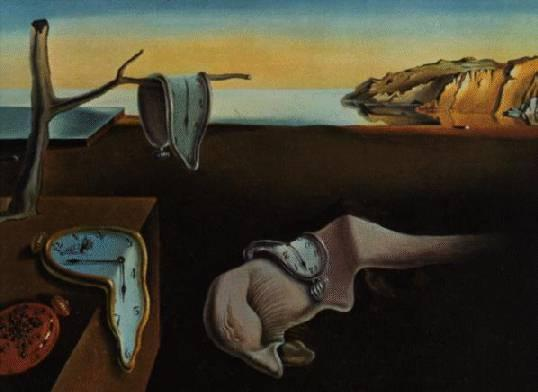
\includegraphics[height=23mm,keepaspectratio]{jsslogo} \hfill
  \parbox[b][23mm]{118mm}{\hrule height 3pt
	   \center{
	   {\fontfamily{pzc} \fontsize{28}{32} \selectfont Journal of Statistical Software}
   \vfill
	   {\it \small \@Month{} \@Year, Volume~\@Volume, \@Seriesname~\@Issue.%
            \hfill \href{http://dx.doi.org/\@DOI}{doi:\,\@DOI}}}\\[0.1cm]
     \hrule height 3pt}}
%</class>
%    \end{macrocode}
%
% This header is then used in the re-defined \verb/\maketitle/:
%    \begin{macrocode}
%<*class>
\if@review
  \renewcommand{\maketitle}{
  \if@nojss
    %% \@oddhead{\@myoddhead}\\[3\baselineskip]
  \else
    \@oddhead{\@myoddhead}\\[3\baselineskip]
  \fi
    {\large
    \noindent
    Reviewer: \@Reviewer
    \vspace{\baselineskip}
    \hrule
    \vspace{\baselineskip}
    \textbf{\@Booktitle}
    \begin{quotation} \noindent
    \@Reviewauthor
    \end{quotation}
    \vspace{0.7\baselineskip}
    \hrule
    \vspace{1.3\baselineskip}
    }

    \thispagestyle{empty}
    \if@nojss
      \markboth{\centerline{\@Shorttitle}}{\centerline{\@Hyperauthor}}
    \else
      \markboth{\centerline{\@Shorttitle}}{\centerline{\@Hypersubject}}
    \fi
    \pagestyle{myheadings}
  }
\else
  \def\maketitle{
  \if@nojss
    %% \@oddhead{\@myoddhead} \par
  \else
    \@oddhead{\@myoddhead} \par
  \fi  
   \begingroup
     \def\thefootnote{\fnsymbol{footnote}}
     \def\@makefnmark{\hbox to 0pt{$^{\@thefnmark}$\hss}}
     \long\def\@makefntext##1{\parindent 1em\noindent
                              \hbox to1.8em{\hss $\m@th ^{\@thefnmark}$}##1}
     \@maketitle \@thanks
   \endgroup
   \setcounter{footnote}{0}

   \if@noheadings
    %% \markboth{\centerline{\@Shorttitle}}{\centerline{\@Hypersubject}}
    \else
     \thispagestyle{empty}
      \if@nojss
        \markboth{\centerline{\@Shorttitle}}{\centerline{\@Hyperauthor}}
      \else
        \markboth{\centerline{\@Shorttitle}}{\centerline{\@Hypersubject}}
      \fi
     \pagestyle{myheadings}
   \fi

   \let\maketitle\relax \let\@maketitle\relax
   \gdef\@thanks{}\gdef\@author{}\gdef\@title{}\let\thanks\relax
  }

  \def\@maketitle{\vbox{\hsize\textwidth \linewidth\hsize
  \if@nojss
    %% \vskip 1in
  \else
    \vskip 1in  
  \fi
   {\centering
   {\LARGE\bf \@title\par}
   \vskip 0.2in plus 1fil minus 0.1in
   {
       \def\and{\unskip\enspace{\rm and}\enspace}%
       \def\And{\end{tabular}\hss \egroup \hskip 1in plus 2fil
   	      \hbox to 0pt\bgroup\hss \begin{tabular}[t]{c}\large\bf\rule{\z@}{24pt}\ignorespaces}%
       \def\AND{\end{tabular}\hss\egroup \hfil\hfil\egroup
   	      \vskip 0.1in plus 1fil minus 0.05in
   	      \hbox to \linewidth\bgroup\rule{\z@}{10pt} \hfil\hfil
   	      \hbox to 0pt\bgroup\hss \begin{tabular}[t]{c}\large\bf\rule{\z@}{24pt}\ignorespaces}
       \hbox to \linewidth\bgroup\rule{\z@}{10pt} \hfil\hfil
       \hbox to 0pt\bgroup\hss \begin{tabular}[t]{c}\large\bf\rule{\z@}{24pt}\@author
       \end{tabular}\hss\egroup
   \hfil\hfil\egroup}
   \vskip 0.3in minus 0.1in
   \hrule
   \begin{abstract}
   \@Abstract
   \end{abstract}}
   \textit{Keywords}:~\@Keywords.
   \vskip 0.1in minus 0.05in
   \hrule
   \vskip 0.2in minus 0.1in
  }}
\fi
%</class>
%    \end{macrocode}
%
% The appearance of sections, subsections and subsubsections is
% controlled by
%    \begin{macrocode}
%<*class>
%% sections, subsections, and subsubsections
\newlength{\preXLskip}
\newlength{\preLskip}
\newlength{\preMskip}
\newlength{\preSskip}
\newlength{\postMskip}
\newlength{\postSskip}
\setlength{\preXLskip}{1.8\baselineskip plus 0.5ex minus 0ex}
\setlength{\preLskip}{1.5\baselineskip plus 0.3ex minus 0ex}
\setlength{\preMskip}{1\baselineskip plus 0.2ex minus 0ex}
\setlength{\preSskip}{.8\baselineskip plus 0.2ex minus 0ex}
\setlength{\postMskip}{.5\baselineskip plus 0ex minus 0.1ex}
\setlength{\postSskip}{.3\baselineskip plus 0ex minus 0.1ex}


\newcommand{\jsssec}[2][default]{\vskip \preXLskip%
  \pdfbookmark[1]{#1}{Section.\thesection.#1}%
  \refstepcounter{section}%
  \centerline{\textbf{\Large \thesection. #2}} \nopagebreak  
  \vskip \postMskip \nopagebreak}
\newcommand{\jsssecnn}[1]{\vskip \preXLskip%
  \centerline{\textbf{\Large #1}} \nopagebreak
  \vskip \postMskip \nopagebreak}

\newcommand{\jsssubsec}[2][default]{\vskip \preMskip%
  \pdfbookmark[2]{#1}{Subsection.\thesubsection.#1}%
  \refstepcounter{subsection}%
  \textbf{\large \thesubsection. #2} \nopagebreak
  \vskip \postSskip \nopagebreak}
\newcommand{\jsssubsecnn}[1]{\vskip \preMskip%
  \textbf{\large #1} \nopagebreak
  \vskip \postSskip \nopagebreak}

\newcommand{\jsssubsubsec}[2][default]{\vskip \preSskip%
  \pdfbookmark[3]{#1}{Subsubsection.\thesubsubsection.#1}%
  \refstepcounter{subsubsection}%
  {\large \textit{#2}} \nopagebreak
  \vskip \postSskip \nopagebreak}
\newcommand{\jsssubsubsecnn}[1]{\vskip \preSskip%
  {\textit{\large #1}} \nopagebreak
  \vskip \postSskip \nopagebreak}

\newcommand{\jsssimplesec}[2][default]{\vskip \preLskip%
%%  \pdfbookmark[1]{#1}{Section.\thesection.#1}%
  \refstepcounter{section}%
  \textbf{\large #1} \nopagebreak
  \vskip \postSskip \nopagebreak}
\newcommand{\jsssimplesecnn}[1]{\vskip \preLskip%
  \textbf{\large #1} \nopagebreak
  \vskip \postSskip \nopagebreak}

\if@review
  \renewcommand{\section}{\secdef \jsssimplesec \jsssimplesecnn}
  \renewcommand{\subsection}{\secdef \jsssimplesec \jsssimplesecnn}
  \renewcommand{\subsubsection}{\secdef \jsssimplesec \jsssimplesecnn}
\else
  \renewcommand{\section}{\secdef \jsssec \jsssecnn}
  \renewcommand{\subsection}{\secdef \jsssubsec \jsssubsecnn}
  \renewcommand{\subsubsection}{\secdef \jsssubsubsec \jsssubsubsecnn}
\fi
%</class>
%    \end{macrocode}
%
% The hypersetup uses some modified colors
%    \begin{macrocode}
%<*class>
%% colors
\definecolor{Red}{rgb}{0.5,0,0}
\definecolor{Blue}{rgb}{0,0,0.5}
%</class>
%    \end{macrocode}
% and is then defined by
%    \begin{macrocode}
%<*class>
\if@review
  \hypersetup{%
    hyperindex = {true},
    colorlinks = {true},
    linktocpage = {true},
    plainpages = {false},
    linkcolor = {Blue},
    citecolor = {Blue},
    urlcolor = {Red},
    pdfstartview = {Fit},
    pdfpagemode = {None},
    pdfview = {XYZ null null null}
  }
\else
  \hypersetup{%
    hyperindex = {true},
    colorlinks = {true},
    linktocpage = {true},
    plainpages = {false},
    linkcolor = {Blue},
    citecolor = {Blue},
    urlcolor = {Red},
    pdfstartview = {Fit},
    pdfpagemode = {UseOutlines},
    pdfview = {XYZ null null null}
  }
\fi
%</class>
%    \end{macrocode}
%
% The information for the hyper summary requires
% some information which has not been processed
% before the beginning of the document. Therefore,
% we need a second \verb/\hypersetup/.
%    \begin{macrocode}
%<*class>
\if@nojss
  \AtBeginDocument{
    \hypersetup{%
      pdfauthor = {\@Hyperauthor},
      pdftitle = {\@Plaintitle},
      pdfkeywords = {\@Plainkeywords}
    }
  }
\else
  \AtBeginDocument{
    \hypersetup{%
      pdfauthor = {\@Hyperauthor},
      pdftitle = {\@Plaintitle},
      pdfsubject = {\@Hypersubject},
      pdfkeywords = {\@Plainkeywords}
    }
  }
\fi
%</class>
%    \end{macrocode}
%
% We put the header at the beginning of the
% document (for footer see above).
%    \begin{macrocode}
%<*class>
\if@notitle
  %% \AtBeginDocument{\maketitle}
\else
  \AtBeginDocument{\maketitle}
\fi
%</class>
%    \end{macrocode}
%
% Finally, some additional commands are provided for writing about
% software (code, programming languages, packages),
%    \begin{macrocode}
%<*class>
%% commands
\newcommand\code{\bgroup\@makeother\_\@makeother\~\@makeother\$\@codex}
\def\@codex#1{{\normalfont\ttfamily\hyphenchar\font=-1 #1}\egroup}
%%\let\code=\texttt
\let\proglang=\textsf
\newcommand{\pkg}[1]{{\fontseries{b}\selectfont #1}}
%</class>
%    \end{macrocode}
% for specifying e-mail addresses,
%    \begin{macrocode}
%<*class>
\newcommand{\email}[1]{\href{mailto:#1}{\normalfont\texttt{#1}}}
%</class>
%    \end{macrocode}
% digital object identifiers (DOIs),
%    \begin{macrocode}
%<*class>
\ifx\csname urlstyle\endcsname\relax
  \newcommand\@doi[1]{doi:\discretionary{}{}{}#1}\else
  \newcommand\@doi{doi:\discretionary{}{}{}\begingroup
\urlstyle{tt}\Url}\fi
\newcommand{\doi}[1]{\href{http://dx.doi.org/#1}{\normalfont\texttt{\@doi{#1}}}}
%</class>
%    \end{macrocode}
% and for mathematical notation.
%    \begin{macrocode}
%<*class>
\newcommand{\E}{\mathsf{E}}
\newcommand{\VAR}{\mathsf{VAR}}
\newcommand{\COV}{\mathsf{COV}}
\newcommand{\Prob}{\mathsf{P}}
%</class>
%    \end{macrocode}
